\documentclass{beamer}
\usepackage{../../shared/styles/custom}
\usepackage{../../shared/styles/conventions}

\mathtoolsset{showonlyrefs}  

%\beamerdefaultoverlayspecification{<+->}


	\ifx\relax#1\relax  \item \else \item[#1] \fi
	\abovedisplayskip=0pt\abovedisplayshortskip=0pt~\vspace*{-\baselineskip}}



\title{Multivariate Normal Distribution I}
\date{\today}
\author{Nipun Batra}
\institute{IIT Gandhinagar}
\begin{document}
  \maketitle
  
  


\begin{frame}{Univariate Normal Distribution}

The probability density of univariate Gaussian is given as: $$f(x) = \frac{1}{\sigma \sqrt{2\pi} } e^{-\frac{1}{2}\left(\frac{x-\mu}{\sigma}\right)^2}$$
	
also, given as 
$$f(x)\sim \mathcal{N}(\mu, \sigma^2)$$

with mean $\mu \in R$ and variance $\sigma^2 >0$ 

\end{frame}

\begin{frame}{Univariate Normal Distribution}
Pop Quiz: Why is the denominator the way it is? Let the normalizing constant be $c$ and let $g(x) = e^{-\frac{1}{2}\left(\frac{x-\mu}{\sigma}\right)^2}$.

\begin{gather}
\visible<1->{1 = \int_{-\infty}^{\infty} c \cdot g(x) dx\\}
\visible<2->{1 = \int_{-\infty}^{\infty} ce^{-\frac{(x - u)^2}{2\sigma^2}} dx}
\end{gather}
\visible<3->{Let's substitute $\frac{x - u}{\sqrt{2}\sigma}$ with $t$.}
\begin{gather}
\visible<4->{1 = \int_{-\infty}^{\infty} ce^{-t^2} dt \times \sqrt{2}\sigma\\}
\visible<5->{1 = \sqrt{2}\sigma c \times 2\int_{0}^{\infty} e^{-t^2} dt}
\end{gather}
\end{frame}

\begin{frame}{Univariate Normal Distribution}
	$$ \frac{2}{\sqrt{\pi}}\int_{0}^{\infty} e^{-t^2} dt $$
	The above expression is called error function and is it's value is denoted by $erf(t)$. In our case, we want $erf(\infty)$ which is equal to 1.
	
	\begin{gather}
	\visible<2->{1 = \sqrt{2\pi}\sigma c \times \frac{2}{\sqrt{\pi}}\int_{0}^{\infty} e^{-t^2} dt\\}
	\visible<3->{1 = \sqrt{2\pi}\sigma c \times 1\\}
	\visible<4->{\frac{1}{\sqrt{2\pi}\sigma} = c}
	\end{gather}
\end{frame}

\begin{frame}{Univariate Normal Distribution}
	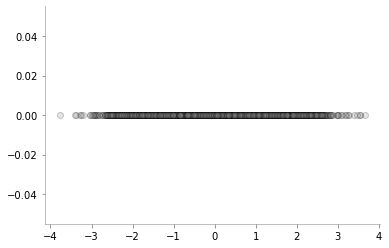
\includegraphics[width=\linewidth,height=\textheight,keepaspectratio]{fig1} 
\end{frame}

\begin{frame}{Univariate Normal Distribution}
	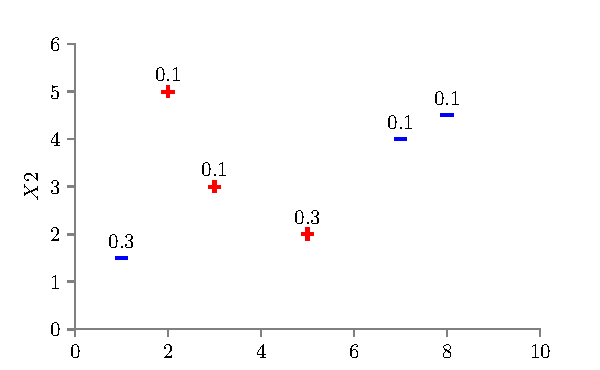
\includegraphics[width=\linewidth,height=\textheight,keepaspectratio]{fig2}
\end{frame}

%\begin{frame}{Univariate Normal Distribution}
%Add plots for 1d histogram with different bin-width
%\end{frame}

\begin{frame}{Univariate Normal Distribution}
	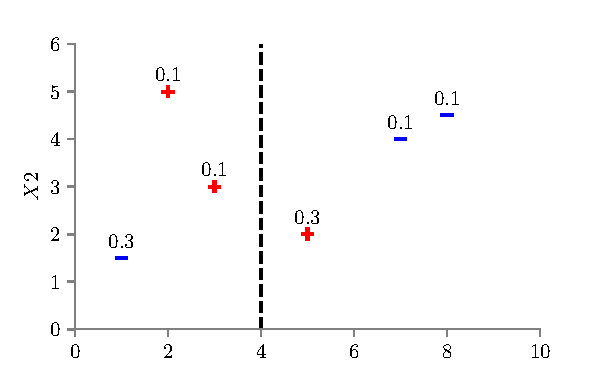
\includegraphics[width=\linewidth,height=\textheight,keepaspectratio]{fig3}
\end{frame}


\begin{frame}{Bivariate Normal Distribution}
Bivariate normal distribution of two-dimensional random vector $\bf{X} =\begin{bmatrix}
X_{1} \\
X_{2} \\
\end{bmatrix}
$

\begin{gather}
	\bf{X} = \begin{pmatrix}
	X_1 \\
	X_2
	\end{pmatrix} \sim \mathcal{N}_2 (\mu , \Sigma)
\end{gather}

where, mean vector $\bm{\mu} =\begin{bmatrix}
\mu_{1} \\
\mu_{2} \\
\end{bmatrix}
=\begin{bmatrix}
\operatorname{E}[X_{1}] \\
\operatorname{E}[X_{2}] \\
\end{bmatrix}
$

and, covariance matrix $\Sigma$
$$\Sigma_{i,j} := \operatorname{E} [(X_i - \mu_i)( X_j - \mu_j)] = \operatorname{Cov}[X_i, X_j] $$
\end{frame}

\begin{frame}{Bivariate Normal Distribution}
	
	\visible<1->{Question: What is Cov(X, X)?}
	
	\visible<2->{Answer: Var(X) = Cov(X, X) =  $\operatorname{E}[(X - \operatorname{E}[X])]^2$}
	
	\visible<2->{In the case of univariate normal, Var(X) is written as $\sigma^2$}
	
	\visible<3->{Question: What is the relation between $\Sigma_{i, j}$ and $\Sigma_{j, i}$?}
	
	\visible<4->{Answer: They are the same!}
	
	\visible<5->{Question: What can we say about the covariance matrix $\Sigma$?}
	
	\visible<6->{Answer: It is symmetric. Thus $\Sigma = \Sigma^T$}
	
\end{frame}

\begin{frame}{Correlation and Covariance}
If $X$ and $Y$ are two random variables, with means (expected values) $\mu_X$ and $\mu_Y$ and standard deviations $\sigma_X$ and $\sigma_Y$, respectively, then their covariance and correlation are as follows:

$$\text{cov}_{XY} = \sigma_{XY} = E[(X-\mu_X)\,(Y-\mu_Y)] $$

\visible<2->{$$	\text{corr}_{XY} = \rho_{XY} = E[(X-\mu_X)\,(Y-\mu_Y)]/(\sigma_X \sigma_Y)
$$}
\visible<3->{so that
$$
\rho_{XY} = \sigma_{XY} / (\sigma_X \sigma_Y) $$

where $E$ is the expected value operator. }
\end{frame}

\begin{frame}{PDF of bivariate normal distribution}

We might have seen that 

$$f_X(X_1, X_2) = \frac{exp(\frac{-1}{2}(X-\mu)^T \Sigma^{-1}(X-\mu))}{2\pi |\Sigma|^\frac{1}{2}}$$

How do we get such a weird looking formula?!

\end{frame}

\begin{frame}{PDF of bivariate normal with no cross-correlation}

Let us assume no correlation between $X_1$ and $X_2$.

We have $\Sigma = \begin{bmatrix}
\sigma_1^2 & 0 \\
0 & \sigma_2^2 \\
\end{bmatrix}$

We have $f_X(X_1, X_2) = f_X(X_1)f_X(X_2)$

$$=\frac{1}{\sigma_1 \sqrt{2\pi} } e^{-\frac{1}{2}\left(\frac{X_1-\mu_1}{\sigma_1}\right)^2} \times \frac{1}{\sigma_2 \sqrt{2\pi} } e^{-\frac{1}{2}\left(\frac{X_2-\mu_2}{\sigma_2}\right)^2}$$

$$= \frac{1}{\sigma_1 \sigma_2 2\pi } e^{-\frac{1}{2}\{\left(\frac{X_1-\mu_1}{\sigma_1}\right)^2 + \left(\frac{X_2-\mu_2}{\sigma_2}\right)^2 \}}  $$
\end{frame}

\begin{frame}{PDF of bivariate normal with no cross-correlation}

Let us consider only the exponential part for now

$ Q =  \left(\frac{X_1-\mu_1}{\sigma_1}\right)^2 + \left(\frac{X_2-\mu_2}{\sigma_2}\right)^2 $

Question: Can you write Q in the form of vectors X and $\mu$?

$$
 = \begin{bmatrix}
	X_1 - \mu_1 &
	X_2 - \mu_2 \\
\end{bmatrix}_{1\times2}  g(\Sigma)_{2\times2} \begin{bmatrix}
X_1 - \mu_1 \\
X_2 - \mu_2 \\
\end{bmatrix}_{2\times1}
$$

Here $g(\Sigma)$ is a matrix function of $\Sigma$ that will result in $\sigma_1^2$ like terms in the denominator; also there is no cross-terms indicating zeros in right diagonal!

$g(\Sigma) = \begin{bmatrix}
 \frac{1}{\sigma_1^2}& 0  \\
 0 &  \frac{1}{\sigma_2^2} \\
\end{bmatrix}_{2\times2} = \frac{1}{\sigma_1^2 \sigma_2^2}\begin{bmatrix}
{\sigma_2^2}& 0  \\
0 &  {\sigma_1^2}   \\ 
\end{bmatrix}_{2\times2} = \frac{1}{|\Sigma|} \operatorname{adj(\Sigma)} = \Sigma^{-1}$
\end{frame}


\begin{frame}{PDF of bivariate normal with no cross-correlation}
Let us consider the normalizing constant part now.
$M = \frac{1}{\sigma_1 \sigma_2 2\pi }$
$=\frac{1}{2\pi \times |\Sigma|^{\frac{1}{2}}}$
\end{frame}

\begin{frame}{Bivariate Gaussian samples with cross-correlation  $\neq$ 0}
	\begin{center}
		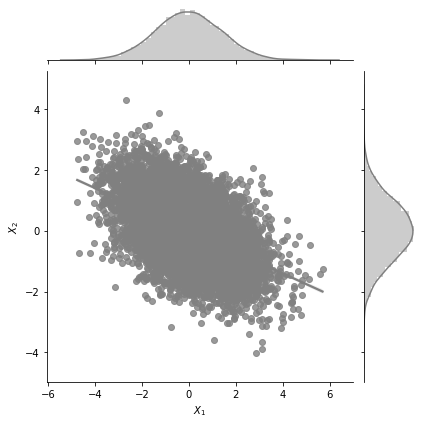
\includegraphics[width=\linewidth,height=\textheight - 10pt,keepaspectratio]{cross-non-zero}
	\end{center}
\end{frame}

\begin{frame}{Bivariate Gaussian samples with cross-correlation  = 0}
	\begin{center}
		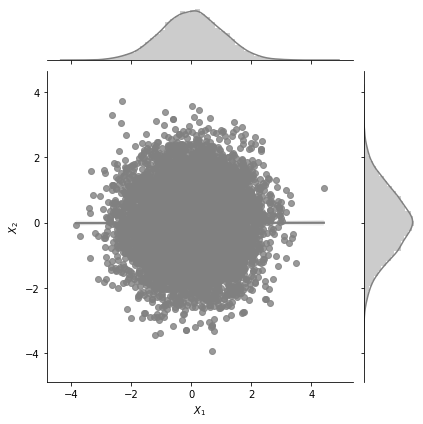
\includegraphics[width=\linewidth,height=\textheight - 10pt,keepaspectratio]{cross-0}
	\end{center}
\end{frame}



\begin{frame}{Intuition for Multivariate Gaussian}
	
	Let us assume no correlation between the elements of $\bf{X}$. This means $\Sigma$ is a diagonal matrix.
	
	We have $\Sigma = \begin{bmatrix} 
	\sigma_{1}^2 & & \textbf{0}\\
	 & \ddots &\\
	\textbf{0} &  & \sigma_n^2 
	\end{bmatrix}
	$ 
	
	And,
	\begin{gather}
		p(\vx ; \mu, \Sigma)=\frac{1}{(2 \pi)^{\frac{n}{2}}|\Sigma|^{\frac{1}{2}}} \exp \left(-\frac{1}{2}(\vx-\mu)^{T} \Sigma^{-1}(\vx-\mu)\right)
	\end{gather}
	
	As seen in the case for univariate Gaussians, we can write the following for the multivariate case,
	
	We have $f_X(X_1, \cdots, X_n) = f_X(X_1)\times \cdots \times f_X(X_n)$
\end{frame}

\begin{frame}{Intuition for Multivariate Gaussian}
	Now,
	$$=\frac{1}{\sigma_1 \sqrt{2\pi} } e^{-\frac{1}{2}\left(\frac{X_1-\mu_1}{\sigma_1}\right)^2} \times \cdots \times \frac{1}{\sigma_n \sqrt{2\pi} } e^{-\frac{1}{2}\left(\frac{X_n-\mu_n}{\sigma_n}\right)^2}$$
	
	$$= \frac{1}{\sigma_1 \cdots \sigma_n (2\pi)^{\frac{n}{2}} } e^{-\frac{1}{2}\{\left(\frac{X_1-\mu_1}{\sigma_1}\right)^2 + \cdots + \left(\frac{X_n-\mu_n}{\sigma_n}\right)^2 \}}  $$
	
	Taking all $\sqrt{2\pi}$ together, we get $(2\pi)^{\frac{n}{2}}$.
	
	Similarly, taking all $\sigma$ together, we get $\sigma_1 \cdots \sigma_n$. Which can be written as $\vert\Sigma\vert^{\frac{1}{2}}$, given the determinant of a digonal matrix is the multiplication of its diagonal elements.
\end{frame}

\begin{frame}
	Now, let us remove the assumption of no covariance among the elements of X
	
	Main idea: A correlated Gaussian is a rotated independent Gaussian\footnote{Neil Lawrence GPSS 2016}
	
	
	Rotate input space using rotation matrix $R$.
	
		\begin{gather}
		p(\vx ; \mu, \Sigma)=\frac{1}{(2 \pi)^{\frac{n}{2}}|\Sigma|^{\frac{1}{2}}} \exp \left(-\frac{1}{2}(\mR^T\vx-R^T\mu)^{T} \Sigma^{-1}(\mR^T\vx-R^T\mu)\right)
	\end{gather}

	
\begin{gather}
	p(\vx ; \mu, \Sigma)=\frac{1}{(2 \pi)^{\frac{n}{2}}|\Sigma|^{\frac{1}{2}}} \exp \left(-\frac{1}{2}(\vx-\mu)^{T} R\Sigma^{-1}R^T(\vx-\mu)\right)
\end{gather}
	
	
\end{frame}

\begin{frame}
	
	$C = R\Sigma^{-1}R^T$
\begin{gather}
	p(\vx ; \mu, \Sigma)=\frac{1}{(2 \pi)^{\frac{n}{2}}|C|^{\frac{1}{2}}} \exp \left(-\frac{1}{2}(\vx-\mu)^{T} C^{-1}(\vx-\mu)\right)
\end{gather}
\end{frame}

\end{document}
